\documentclass{article}
\usepackage[russian]{babel}
\usepackage[utf8]{inputenc}
\usepackage{amsfonts}
\usepackage{amssymb}
\usepackage{listings}
\usepackage{amsmath}
\usepackage{amsthm}
\usepackage{minted}
\usepackage{indentfirst}
\usepackage{hyperref}
\usepackage{cleveref}
\usepackage{graphicx}
\usepackage{wrapfig}
\usepackage{tikz}
\usepackage{ragged2e}
\usepackage{multirow}
\usepackage{subfig}

\title{СМВМ, задание №2}
\author{Болохонов Артем Владимирович}

\begin{document}

\date{}
\maketitle

\textbf{Описание задания:} для приближения в ячейке использовались полиномы Чебышева 5 степени, глобальная СЛАУ решалась методом. Программа решалась на языке программирования \textit{Python}.


Расчеты проводились на компьютере AMD Ryzen 7 7700x 4.5GHz (up to 5.4 GHz), 8 cores; DIMM DDR5 32 Gb 6000 MHz.


\begin{table}[H]
\centering
\begin{tabular}{|c|l|l|l|l|l|l|}
\hline
K   & \multicolumn{1}{c|}{$||E_a||_\infty$} & \multicolumn{1}{c|}{R} & \multicolumn{1}{c|}{$||E_r||_\infty$} & \multicolumn{1}{c|}{R} & \multicolumn{1}{c|}{$t_{sol}$} & \multicolumn{1}{c|}{$\mu(\tilde{A})$} \\ \hline
5   & 6.20e-02                              & ------                      & 6.94e-03                              & ------                      & 3.40e-04                       & 8.34e+03                              \\ \hline
10  & 1.58e-02                              & 1.97               & 1.70e-03                              & 2.03               & 2.67e-04                       & 1.27e+05                              \\ \hline
20  & 3.98e-03                              & 1.99               & 4.21e-04                              & 2.01               & 1.64e-03                       & 2.02e+06                              \\ \hline
40  & 9.95e-04                              & 2.00               & 1.05e-04                              & 2.00               & 1.39e-02                       & 3.24e+07                              \\ \hline
80  & 2.49e-04                              & 2.00               & 2.63e-05                              & 2.00               & 4.70e-02                       & 5.18e+08                              \\ \hline
160 & 6.22e-05                              & 2.00               & 6.56e-06                              & 2.00               & 2.09e-01                       & 8.28e+09                              \\ \hline
\end{tabular}
\caption{\centeringрезультаты численных экспериментов в случае решения глобальной СЛАУ прямым методом}
\end{table}

\begin{figure}[H]
  \centering
  \subfloat{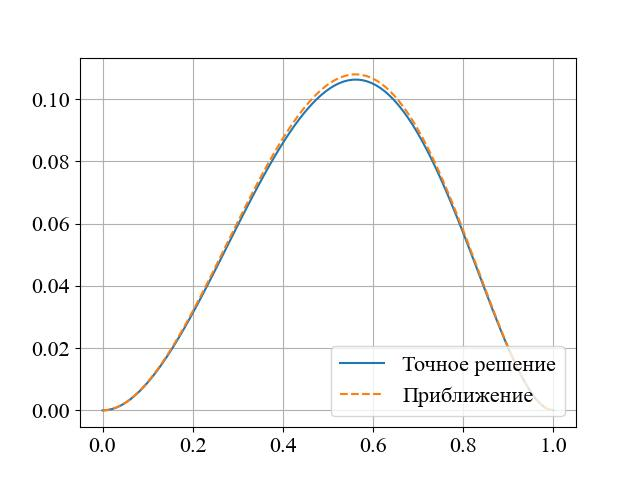
\includegraphics[width=0.5\textwidth]{10.jpeg}}
  \hfill
  \subfloat{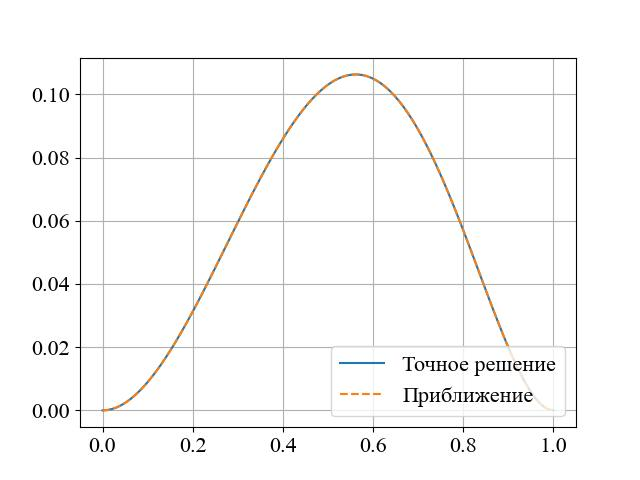
\includegraphics[width=0.5\textwidth]{80.jpeg}}
  \caption{\centeringсравнение точного и приближенного решения с $K = 10$ и $K = 80$}
\end{figure}

Ответы на вопросы:
\begin{enumerate}
    \item \textit{Оцените арифметическую сложность решения глобальной СЛАУ?} \\
    ~$\operatorname{O}(K \cdot N^2)$.
    \item \textit{Почему нельзя напрямую решить каждую локальную СЛАУ один раз, не составляя глобальной СЛАУ?} \\
    Решая локальную матрицу мы потеряем условие согласования для соседней ячейки, тем самым мы потеряем непрерывность линейной комбинации. Если же начать добавлять условия согласования мы итеративно получим глобальную СЛАУ.
    \item \textit{Как можно учесть разреженность матрицы глобальной СЛАУ при ее решении?} \\
    Это позволяет использовать специализированные методы решения для разреженных матриц.
\end{enumerate}
\end{document}
